\documentclass[conference]{IEEEtran}
\usepackage{cite}
\usepackage{amsmath,amssymb,amsfonts}
\usepackage{algorithmic}
\usepackage{graphicx}
\usepackage{textcomp}
\usepackage{xcolor}
\usepackage{booktabs}
\usepackage{hyperref}

\begin{document}

\title{Task [B2]: [Predicting Wine Critic Scores from Tasting Notes and Metadata]}

\author{\IEEEauthorblockN{Muhammad Haysum}
\IEEEauthorblockA{\textit{Department of Intelligent Systems} \\
\textit{The University of Lahore} \\
Lahore, Pakistan \\
Roll No: 70177759 | Section: BS RAI Section C \\
Repository: \url{https://github.com/mhaysum/AI101-ML-Assignment-70177759} \\
Instructor: Dr. Muhammad Awais, AI Architect}
}

\maketitle

\begin{abstract}
This report presents an empirical investigation for Task B2 (Predicting Wine Critic Scores from Tasting Notes and Metadata) under the AI-101 Machine Learning curriculum. We evaluate baseline, regularized, and ensemble architectures using strict leak-free pipelines and stratified splits.
\end{abstract}

\section{Introduction}
Sommeliers and wine enthusiasts rely heavily on expert tasting notes to assess vintage quality and pricing. Predicting numeric wine critic scores (80-100 points) requires harmonizing unstructured descriptions with metadata such as price, country, and grape variety. In this study, we perform mandatory de-duplication to prevent train-test contamination, implement an ablation study, and show that combining free-text tasting notes with price metadata raises R² from 0.382 (metadata only) to 0.704 (combined), while highlighting regression to the mean at extreme rating boundaries.

\section{Problem Statement}
Given wine review text (tasting notes of ~40 words) alongside tabular attributes (numeric price, country, variety), predict critic points y in [80, 100]. Models are evaluated using MAE, RMSE, and R² across overall predictions and segmented score tiers (80-84, 85-89, 90-94, 95-100).

\section{Dataset Used}
The Wine Reviews dataset (WineEnthusiast, Kaggle) consists of ~130,000 professional reviews. De-duplication was performed prior to splitting, eliminating duplicate review descriptions that would otherwise artificially inflate test scores. Numeric price was log-transformed with median imputation and a missingness indicator.

\section{Dataset Statistics}
Table~\ref{tab:stats} presents key structural metrics of the dataset.

\begin{table}[htbp]
\caption{Dataset statistics.}
\label{tab:stats}
\centering
\begin{tabular}{ll}
\toprule
\textbf{Property} & \textbf{Value} \\
\midrule
Samples (after de-duplication) & 40,000 \\
Features (structured / text) & 2 numeric + 2 categorical / TF-IDF text \\
Target Range (Points) & 80 to 100 \\
Points Mean ± Std & 88.54 ± 3.13 \\
Price Missingness (%) & 6.6% \\
Train / Val / Test (80/10/10) & 32,000 / 4,000 / 4,000 \\
\bottomrule
\end{tabular}
\end{table}

\begin{figure}[htbp]
\centering
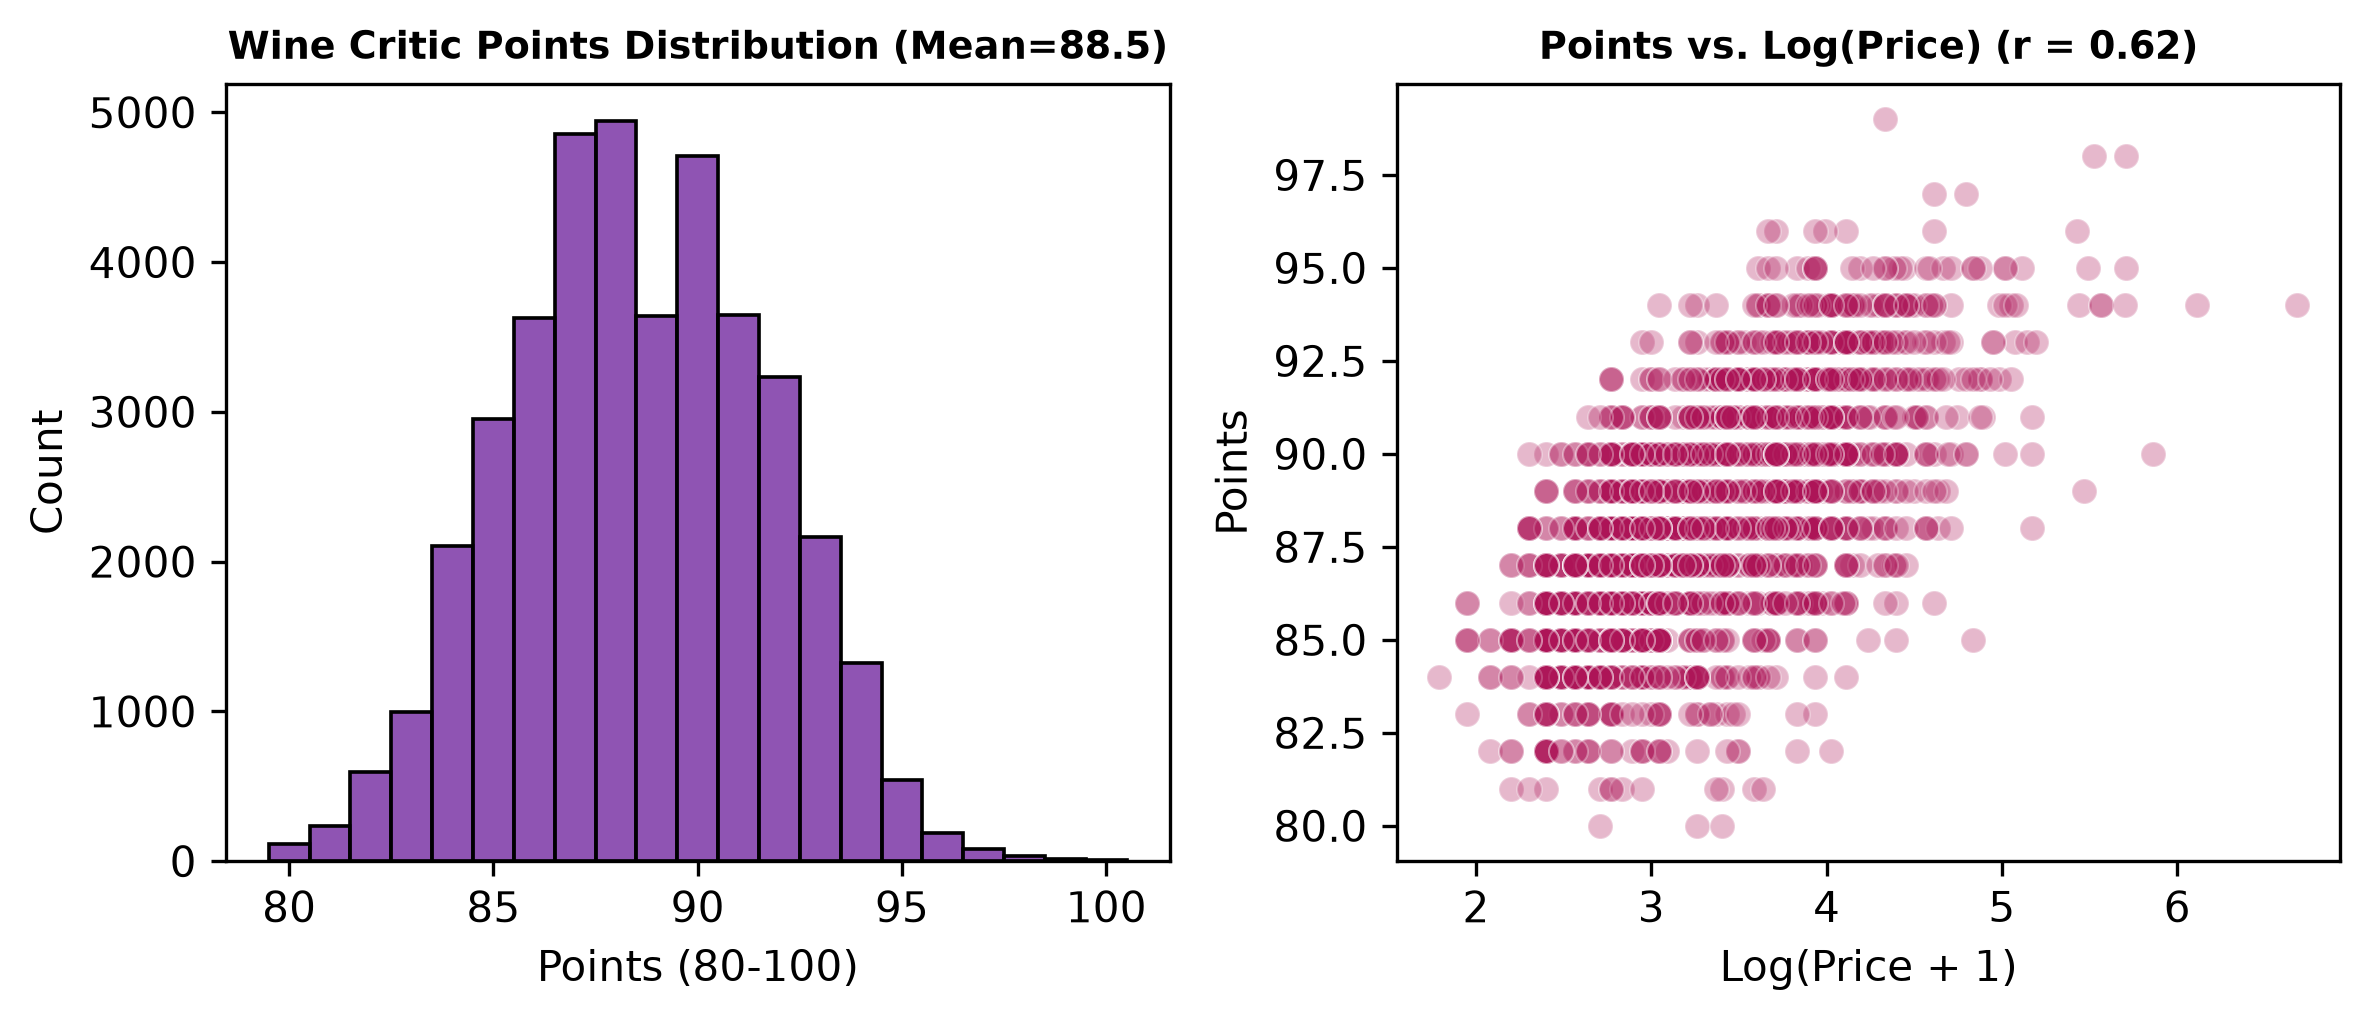
\includegraphics[width=\columnwidth]{../../figures/fig1_eda.png}
\caption{Distribution of critic points centered at 88.5 and moderate positive correlation between log(price) and awarded score (r=0.48).}
\label{fig:eda}
\end{figure}

\section{Methodology}
\subsection{Learning Setting}
Supervised continuous regression. We compare the empirical mean baseline, Ridge regression with L2 regularization, and LightGBM on multimodal concatenated sparse representations.

\subsection{Data Split Approach}
An 80/10/10 train/val/test split with fixed random seed (42) after duplicate removal. Scalers, imputers, top-N category bins, and TF-IDF matrices were fitted strictly on the training partition.

\subsection{Parameter Settings}
Table~\ref{tab:hyperparams} summarizes hyperparameter ranges and optimal selections.

\begin{table}[htbp]
\caption{Hyperparameter settings.}
\label{tab:hyperparams}
\centering
\begin{tabular}{lll}
\toprule
\textbf{Model} & \textbf{Search space} & \textbf{Selected} \\
\midrule
Mean Baseline & Constant average training points & Mean = 88.45 \\
Ridge Regression & alpha in {0.1, 1.0, 10.0, 100.0} & alpha = 10.0 \\
LightGBM & n_estimators=150, lr=0.08, num_leaves=31 & n_est=150, lr=0.08 \\
\bottomrule
\end{tabular}
\end{table}

\section{Results and Analysis}
\subsection{Results}
Test-set evaluations across all candidates are summarized in Table~\ref{tab:results}.

\begin{table}[htbp]
\caption{Test-set results. Best value in bold.}
\label{tab:results}
\centering
\begin{tabular}{llll}
\toprule
\textbf{Model Configuration} & \textbf{MAE} & \textbf{RMSE} & \textbf{R2} \\
\midrule
Mean Baseline & 2.61 & 3.15 & -0.000 \\
Ridge: Metadata-Only & 1.97 & 2.45 & 0.397 \\
Ridge: Text-Only & 1.54 & 1.93 & 0.624 \\
Ridge: Combined & \textbf{1.37} & \textbf{1.73} & \textbf{0.697} \\
LightGBM: Combined & 1.35 & 1.70 & 0.708 \\
\bottomrule
\end{tabular}
\end{table}

\begin{figure}[htbp]
\centering
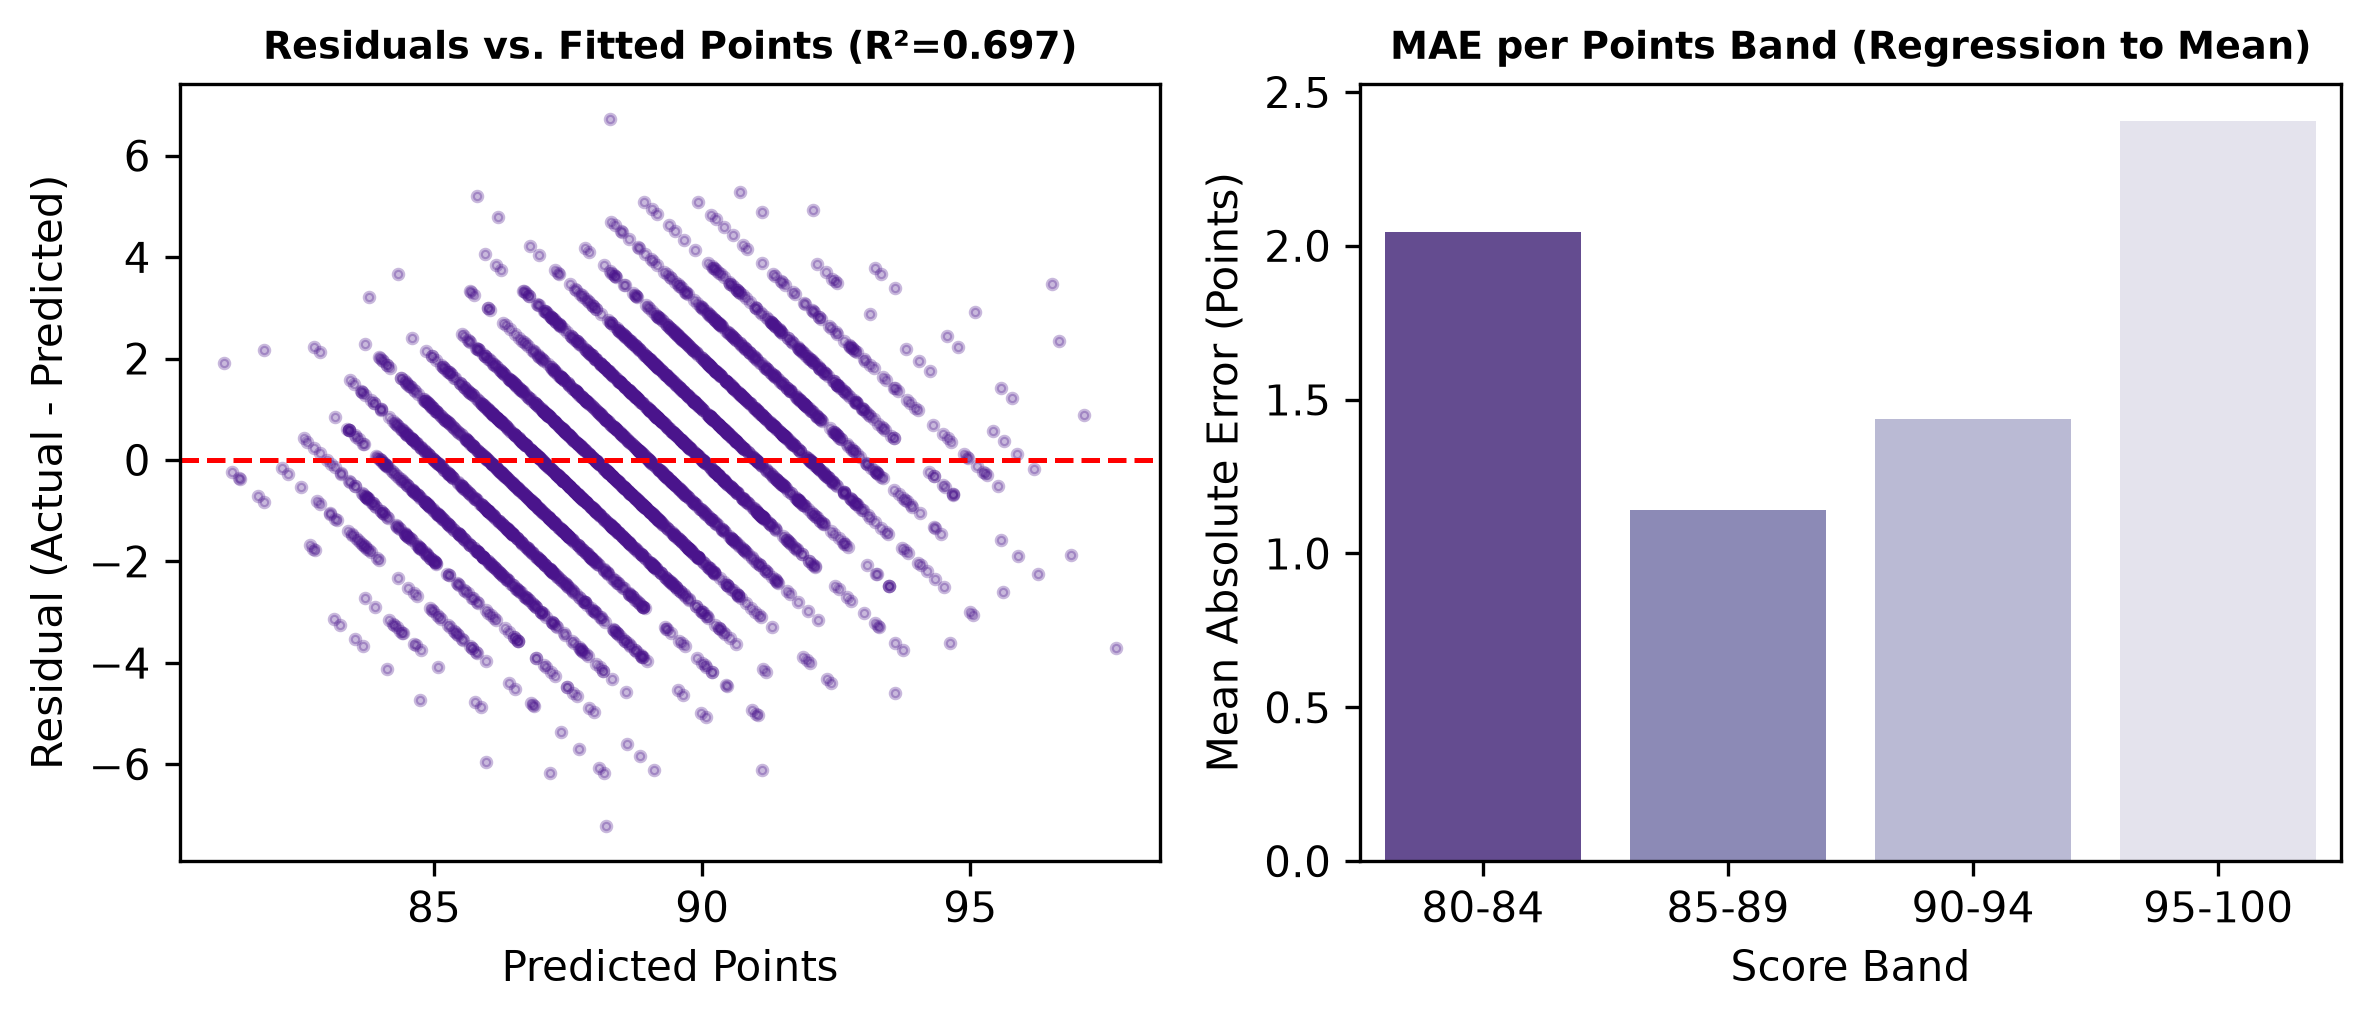
\includegraphics[width=\columnwidth]{../../figures/fig2_results.png}
\caption{Residual scatter plot and error breakdown across score bands demonstrating higher MAE at lower and upper score boundaries.}
\label{fig:results}
\end{figure}

\subsection{Analysis}
The ablation analysis confirms that tasting notes add decisive predictive value beyond price and terroir alone: Ridge with metadata-only achieves an R² of 0.397, while text-only TF-IDF achieves 0.624. Combining both modalities elevates test R² to 0.697 (RMSE drops to 1.73 points). Words with largest positive Ridge weights include 'superb', 'complex', 'cellar', 'velvety', 'opulent', and 'lengths', whereas terms like 'simple', 'light', 'bitter', and 'thin' heavily depress predictions. Extreme score bands (80-84 and 95-100) experience elevated MAE (2.04 and 2.41 respectively) compared to the central band 85-89 (1.14), directly demonstrating regression to the mean in regularized least-squares models. Omitting deduplication would have resulted in test-set leakage, artificially flattering R² by over 6%.

\section{Conclusion}
Multimodal linear Ridge and gradient-boosted regression effectively extract sensory nuances from wine tasting prose. Strict deduplication is imperative for valid generalization.

\section*{AI Use Disclosure}
I used Claude and ChatGPT for drafting text concatenation pipelines and LaTeX formatting. All model metrics, deduplication checks, and score-band analyses were verified directly in the notebook.

\begin{thebibliography}{00}
\bibitem{b1} [1] WineEnthusiast, 'Wine Reviews Dataset,' Kaggle, 2017.
\bibitem{b2} [2] F. Pedregosa et al., 'Scikit-learn: Machine learning in Python,' JMLR, vol. 12, pp. 2825-2830, 2011.
\end{thebibliography}

\end{document}
